% --- [ Front-end Components ] -------------------------------------------------

\subsection{Front-end Components}

% TODO: Rewrite and clarify.

The front-end module is responsible for converting the input into LLVM IR. Two common scenarios exists, converting binary files (e.g. executables, shared libraries and relocatable object code) and converting source code (e.g. C, Haskell, Rust, …) into LLVM IR. The first scenario is presented in figure \ref{fig:front-end_binary} and the second in figure \ref{fig:front-end_source}.

% TODO: Mention opt --mem2reg.

\begin{figure}[htbp]
	\begin{center}
		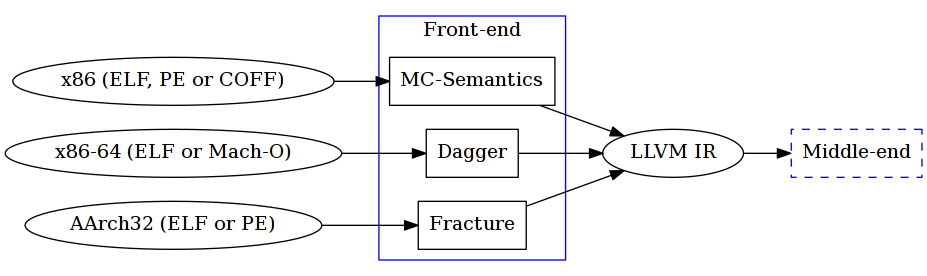
\includegraphics[width=\textwidth]{inc/front-end_binary.png}
		\caption{The three open source projects MC-Semantics, Dagger and Fracture translate native code of various architectures (e.g. x86, x86-64 and ARM) and file formats (e.g. ELF, PE, COFF and Mach-o) to LLVM IR.}
		\label{fig:front-end_binary}
	\end{center}
\end{figure}

\begin{figure}[htbp]
	\begin{center}
		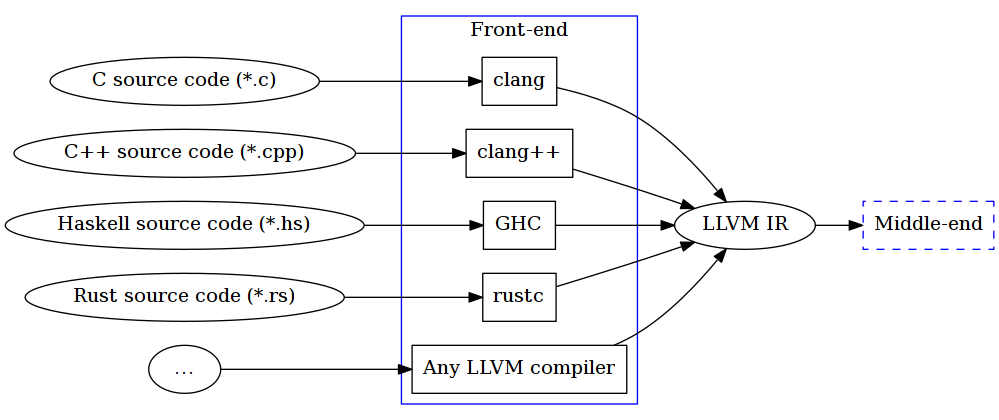
\includegraphics[width=\textwidth]{inc/front-end_source.png}
		\caption{Several open source compilers translate high-level programming languages to LLVM IR. Three such compilers are Clang, the Glasgow Haskell Compiler and the Rust compiler which translate C, Haskell and Rust respectively to LLVM IR.}
		\label{fig:front-end_source}
	\end{center}
\end{figure}
